\documentclass{zjureport}

\usepackage{hyperref}
\hypersetup{
    colorlinks=true,
}
\usepackage{float} 


\major{地理信息科学} %专业
\name{路人甲} %名字
\stuid{3230106666} %学号
\college{地球科学学院} %学院
\score{100} %成绩
\teacher{路人乙} %教师签字
\course{GIS平台实践} %课程名称
\lab{空间数据探索} %实验名称
\TA{路人乙} %指导老师
\expname{路人甲,路人乙,路人丙} %实验人
\LABdate{\today} %日期


\begin{document}

\makeheader

\section{实验目的和要求}
\subsection{实验目的}
掌握ArcGIS Pro 矢量空间分析基本方法。

\subsection{实验要求}
独立完成实验,将实验内容2)的解题思路、解题步骤、解题结果与分析撰写
成实验报告。


\section{实验内容和步骤}

\subsection{实验内容}

\begin{enumerate}
    \item 完成教程第6章6.1节-6.4节内容的上机操作。
    \item 基于实验二----实验五,完成以下实验内容:
    \begin{enumerate}
        \item 将三江水域及其岸上50米范围划为三江河湖滨岸保护带。
        \item 将水库水域周围200米范围内的陆域划为水库饮用水水源一级保护区。
        \item 在将风景名胜区、森林公园核心保护区、水库饮用水水源一级保护区和三江河湖滨岸保护带作叠加分析基础上,划分禁止开发区域,并保证禁止开发区域落在研究区范围内。
        \item 分乡镇统计各类禁止开发区域人类活动用地规模。
    \end{enumerate}
\end{enumerate}

\subsection{实验原理}
矢量空间分析。 


\section{主要仪器设备}
计算机和ArcGIS Pro软件

\section{实验步骤和记录}
\subsection{(一)三江河湖滨岸保护带}
\subsubsection{解题思路}临近三江水域50米距离的区域属于三江河湖滨岸保护带,此时使用
【缓冲区】工具可以生成相应区域的缓冲区,即为三江河湖滨岸保护带。

\subsubsection{解题步骤}
\begin{enumerate}
    \item 单击【分析工具】工具箱中的【邻近分析】|【缓冲区】工具,打开工具窗格,如图设置参数,点击【运行】
\end{enumerate}

\begin{figure}[H]
    \centering
    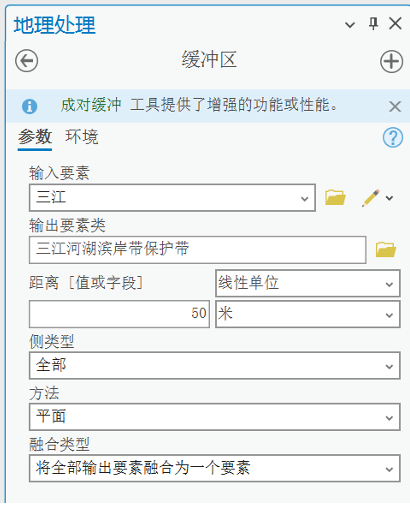
\includegraphics[width=0.5\textwidth]{image/example.png}
    \caption{缓冲区工具}
    \label{fig:buffer}
\end{figure}



\section{实验结果和分析}

\begin{lstlisting}[language=python]
# coding=utf-8
import arcpy
import sys
#read data
data=arcpy.FeatureSet("example.shp”)

\end{lstlisting}

\section{讨论}
讨论讨论讨论讨论讨论讨论讨论讨论讨论讨论讨论讨论

\end{document}
